%
% One column figure
%-----------------------------------------------------------
   \begin{figure}
   \centering
\tikzstyle{smallfig}=[scale=0.25]
   %
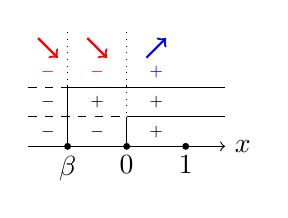
\begin{tikzpicture}[style=smallfig]
\draw[thin,->] (0,0) -- (10,0) node[right] {$x$};

\draw[dotted,thin,-] (2,0) -- (2,6);
\draw[dotted,thin,-] (5,0) -- (5,6);

\draw[dashed,thin,-] (0,1.5) -- (5,1.5);
\draw[thin,-] (5,1.5) -- (10,1.5);
\draw[thin,-] (5,0) -- (5,1.5);

\draw[dashed,thin,-] (0,3) -- (2,3);
\draw[thin,-] (2,3) -- (10,3);
\draw[thin,-] (2,0) -- (2,3);

\node[] at (1,0.75) {\tiny $-$};
\node[] at (3.5,0.75) {\tiny $-$};
\node[] at (6.5,0.75) {\tiny $+$};

\node[] at (1,2.25) {\tiny $-$};
\node[] at (3.5,2.25) {\tiny $+$};
\node[] at (6.5,2.25) {\tiny $+$};

\node[red] at (1,3.75) {\tiny $-$};
\node[red] at (3.5,3.75) {\tiny $-$};
\node[blue] at (6.5,3.75) {\tiny $+$};

\draw[thick,->, red] (0.5,5.5) -- (1.5,4.5);
\draw[thick,->, red] (3,5.5) -- (4,4.5);
\draw[thick,->, blue] (6,4.5) -- (7,5.5);

\fill (2,0) circle (5pt) node[below] {$\beta$};
\fill (5,0) circle (5pt) node[below] {$0$};
\fill (8,0) circle (5pt) node[below] {$1$};
\end{tikzpicture}
\quad
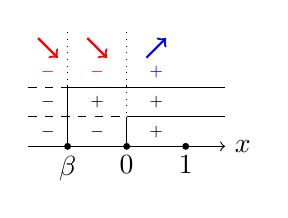
\begin{tikzpicture}[style=smallfig]
\draw[thin,->] (0,0) -- (10,0) node[right] {$x$};

\draw[dotted,thin,-] (2,0) -- (2,6);
\draw[dotted,thin,-] (5,0) -- (5,6);

\draw[dashed,thin,-] (0,1.5) -- (5,1.5);
\draw[thin,-] (5,1.5) -- (10,1.5);
\draw[thin,-] (5,0) -- (5,1.5);

\draw[dashed,thin,-] (0,3) -- (2,3);
\draw[thin,-] (2,3) -- (10,3);
\draw[thin,-] (2,0) -- (2,3);

\node[] at (1,0.75) {\tiny $-$};
\node[] at (3.5,0.75) {\tiny $-$};
\node[] at (6.5,0.75) {\tiny $+$};

\node[] at (1,2.25) {\tiny $-$};
\node[] at (3.5,2.25) {\tiny $+$};
\node[] at (6.5,2.25) {\tiny $+$};

\node[red] at (1,3.75) {\tiny $-$};
\node[red] at (3.5,3.75) {\tiny $-$};
\node[blue] at (6.5,3.75) {\tiny $+$};

\draw[thick,->, red] (0.5,5.5) -- (1.5,4.5);
\draw[thick,->, red] (3,5.5) -- (4,4.5);
\draw[thick,->, blue] (6,4.5) -- (7,5.5);

\fill (2,0) circle (5pt) node[below] {$\beta$};
\fill (5,0) circle (5pt) node[below] {$0$};
\fill (8,0) circle (5pt) node[below] {$1$};
\end{tikzpicture}
\quad
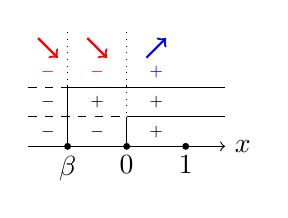
\begin{tikzpicture}[style=smallfig]
\draw[thin,->] (0,0) -- (10,0) node[right] {$x$};

\draw[dotted,thin,-] (2,0) -- (2,6);
\draw[dotted,thin,-] (5,0) -- (5,6);

\draw[dashed,thin,-] (0,1.5) -- (5,1.5);
\draw[thin,-] (5,1.5) -- (10,1.5);
\draw[thin,-] (5,0) -- (5,1.5);

\draw[dashed,thin,-] (0,3) -- (2,3);
\draw[thin,-] (2,3) -- (10,3);
\draw[thin,-] (2,0) -- (2,3);

\node[] at (1,0.75) {\tiny $-$};
\node[] at (3.5,0.75) {\tiny $-$};
\node[] at (6.5,0.75) {\tiny $+$};

\node[] at (1,2.25) {\tiny $-$};
\node[] at (3.5,2.25) {\tiny $+$};
\node[] at (6.5,2.25) {\tiny $+$};

\node[red] at (1,3.75) {\tiny $-$};
\node[red] at (3.5,3.75) {\tiny $-$};
\node[blue] at (6.5,3.75) {\tiny $+$};

\draw[thick,->, red] (0.5,5.5) -- (1.5,4.5);
\draw[thick,->, red] (3,5.5) -- (4,4.5);
\draw[thick,->, blue] (6,4.5) -- (7,5.5);

\fill (2,0) circle (5pt) node[below] {$\beta$};
\fill (5,0) circle (5pt) node[below] {$0$};
\fill (8,0) circle (5pt) node[below] {$1$};
\end{tikzpicture}
   %
   \caption{Showing the how the constraints on $f$ define its shape
   in $[0,1] \times [0,1]$. The first picture shows the regione where $f$
   can lay, the middle one shows tangent in $x=0$ and the condition
   of crossing in $(1,0)$. The rightmost picture shows possible
   shapes of $f$: note how the concavity cannot be pointing upwards.}
   \label{fig:fshape}
   \end{figure}
%-----------------------------------------------------------
%